% \documentclass[sigconf,natbib=false,authordraft]{acmart}
\documentclass[sigconf,natbib=false]{acmart}

% References
\usepackage[style=ACM-Reference-Format,backend=bibtex,sorting=none]{biblatex}
\addbibresource{references.bib}

\usepackage{booktabs}

\usepackage{tikz}
\usetikzlibrary{shapes.geometric, arrows}
\tikzstyle{item} = [rectangle, minimum width=3cm, minimum height=1cm,text centered, draw=black, fill=gray!50]
\tikzstyle{arrow} = [thick,->,>=stealth,shorten <= 1.5pt,shorten >= 1.5pt]

% ACM License Text
\setcopyright{acmcopyright}

% DOI
% \acmDOI{10.475/123_4}

% ISBN
% \acmISBN{123-4567-24-567/08/06}

% Conference Details
% \acmConference[WOODSTOCK'19]{ACM Woodstock conference}{July 2019}{El Paso, Texas USA}

% Year
\acmYear{2020}

% Copyright Year
\copyrightyear{2020}

\title{Comparison of CORD-19-trained GPT-2-based Chatbot Responses Across
  Different Text Semantic Similarity Approaches}

\author{David Oniani}
\affiliation{%
  \institution{Mayo Clinic}
  \department{Kern Center for the Science of Health Care Delivery}
  \city{Rochester}
  \state{MN}
  \country{USA}}
\email{oniani.david@mayo.edu}

\author{Dr.~Yanshan Wang}
\affiliation{%
  \institution{Mayo Clinic}
  \department{Division of Digital Health Sciences}
  \city{Rochester}
  \state{MN}
  \country{USA}}
\email{wang.yanshan@mayo.edu}

\begin{document}

%%%%%%%%%%%%%%%%%%%%%%%%%%%%%%%%%%%%%%%%%%%%%%%%%%%%%%%%%%%%%%%%%%%%%%%%%%%%%%%
% Abstract
%%%%%%%%%%%%%%%%%%%%%%%%%%%%%%%%%%%%%%%%%%%%%%%%%%%%%%%%%%%%%%%%%%%%%%%%%%%%%%%

\begin{abstract}
On March 16 (2020), per request of the White House Office of Science and
Technology Policy, new COVID-19 machine readable dataset
(CORD-19)~\cite{whitehousecovid2020} has been released. Yet, there still was a
need for making this dataset more interpretable and understandable for the
general audience. Besides, there was an urgent need of fast and efficient
information exchange. To accomplish this goal, we built an interactive chatbot
that answers questions related to COVID-19. This not only made the information
from the CORD-19 dataset more understandable to the general audience, but also
put it into real-world use and helped efficiently obtain information concerning
COVID-19. We have utilized 774M GPT-2~\cite{radford2019language} model and
applied transfer learning to retrain the model on the CORD-19 corpus.
Ultimately, we have created an interactive COVID-19 conversational chatbot. In
order to improve the performance of the chatbot, we have applied 4 different
text semantic similarity techniques using pre-trained models including
BERT~\cite{turc2019}, BioBERT~\cite{btz682}, and Universal Sentence Encoder
(USE)~\cite{use} as layers on top of GPT-2-based chatbot. For performance
evaluation purposes, we have asked experienced personnel at Mayo Clinic to rate
our answers and also present these annotations in the paper. Additionally, we
have created a user-friendly interactive web application to be hosted online
and made available for anyone to get more information regarding COVID-19. Our
work has produced good results in both designing a chatbot that produces
high-quality answers to COVID-19-related questions (hence, improving COVID-19
information exchange) and comparing the performance of several embedding
generation and vectorization techniques in the biomedical domain.

\end{abstract}

\keywords{gpt-2, covid-19, cord-19, bert, biobert, universal sentence encoder, tf-idf
  dataset, nlp, ai, semantic similarity}

\maketitle

%%%%%%%%%%%%%%%%%%%%%%%%%%%%%%%%%%%%%%%%%%%%%%%%%%%%%%%%%%%%%%%%%%%%%%%%%%%%%%%
% Introduction
%%%%%%%%%%%%%%%%%%%%%%%%%%%%%%%%%%%%%%%%%%%%%%%%%%%%%%%%%%%%%%%%%%%%%%%%%%%%%%%

\section{Introduction}

COVID-19/Novel coronavirus is an infectious disease caused by severe acute
respiratory syndrome coronavirus 2 (SARS-CoV-2). It was first identified in
December of 2019 in Wuhan, China, and has since spread globally, resulting in
an unprecedented pandemic. As of 17 May 2020, more than 4.66 million cases have
been reported across 188 countries and territories, resulting in more than
312,000 deaths. The White House Office of Science and Technology Policy has
requested a COVID-19 machine readable dataset, now known as CORD-19. Since its
rapid emergence started, many countries have declared the state of emergency
and the need for fast and efficient information sharing as well as tracking
progress related to COVID-19 became crucial. For addressing these issues, we
decided to use CORD-19 for designing a chatbot that would answer questions
related to COVID-19. The chatbot would not only help improve information
sharing, but also as a knowledge base for COVID-19.

\bigskip

\noindent A chatbot is a software which is able to conduct a conversation via
text and/or other means. It is designed to emulate the way people communicate
and give a sense that the conversation only involves humans. Therefore, cutting
edge chatbots can hold a human-level conversation and usually, the performance
of the chatbot is measured via the quality of its responses to humans. Chatbots
have been much studied in recent years and with the advancements in the fields
of artificial intelligence (AI) and natural language processing (NLP), both the the
functionality and the performance have seen drastic improvements. Semantic
similarity of texts, on the other hand, has been studied for a long time and
recent breakthroughs allowed for development of new models such as BERT,
BioBERT, and Universal Sentence Encoder. Today, one of the state-of-the art
conversational artificial intelligence models is GPT-2. GPT-2 is a pre-trained
model, so we have applied transfer learning utilizing CORD-19 for retraining
purposes. The resulted chatbot gave irregularly long responses that would not
be typical of a human. We have therefore decided to further filter the
responses via applying embedding generation algorithms and models such as
tf-idf, BERT, BioBERT, and Universal Sentence Encoder (USE) and then using
semantic similarity approaches such as cosine similarity and inner product. In
other words, we first let a human ask a question and make GPT-2 come up with an
answer. We the further processed the response` with additional filters and
ultimately, applied an embedding generation model for finding the sentences
that are most relevant to the question.

\bigskip

\noindent Our study has produced a chatbot that is both performant and
extensible. Additional layer of filters have shown success in classifying
sentences. The chatbot is also able to be retrained and readjusted to new data,
in case there are new discoveries and scientific achievements related to
COVID-19. Furthermore, chatbot responses have been annotated by experienced
staff at Mayo Clinic and the resuts were consistent across the annotators.

\bigskip

\noindent We will proceed by discussing the related work and the efforts that
have been made previously. A few sections will be dedicated to specific
approaches and materials used in this work. We will discuss the chatbot
evaluation strategy as well as present the annotation results. Finally, we will
also discuss the web-based tool designed to be used with this chatbot the
source code of which (alongside with everything discussed) has been made
available online.

%%%%%%%%%%%%%%%%%%%%%%%%%%%%%%%%%%%%%%%%%%%%%%%%%%%%%%%%%%%%%%%%%%%%%%%%%%%%%%%
% Related Work
%%%%%%%%%%%%%%%%%%%%%%%%%%%%%%%%%%%%%%%%%%%%%%%%%%%%%%%%%%%%%%%%%%%%%%%%%%%%%%%

\section{Related Work}

In the GPT-2 domain, some efforts were made by Wang et al.~\cite{gpt2-ad} where GPT-2
was retrained in order to automatically generate answers to AD-related consumer
questions posted by caregivers and evaluate how good  AI is at answering those
questions. Lee and Hsiang~\cite{lee-hsiang} have fine-tuned GPT-2 for
generating patent claims.  Klein and Nabi~\cite{klein-nabi} have applied GPT-2
in conjunction with BERT for automatic questin generation purposes. We are
unaware of the work which applied 775M GPT-2 model for transfer learning
purposes on the CORD-19 dataset.

\bigskip

\noindent In regard to the work related to comparing pre-trained AI models,
Jin et al. have made some efforts conducting probing experiments and comparing
BERT, ELMo~\cite{elmo}, and BioBERT. Sharma and Daniel~\cite{bioflair} compared
the performance of BERT networks to that of FLAIR~\cite{akbik2018coling}.

\bigskip

\noindent In the general artificial intelligence based chatbot domain, Serbal et al.
~\cite{reinforce-chatbot} have applied deep reinforcement learning for building a
conversational AI chatbot. Adiwardana et al.~\cite{toward-human-chatbot} have developed
a multi-turn open-domain chatbot trained end-to-end on data mined social media conversations.
Yin et al.~\cite{therapy-chatbot} have developed a deep learning based chatbot for
psychological therapy purposes.

%%%%%%%%%%%%%%%%%%%%%%%%%%%%%%%%%%%%%%%%%%%%%%%%%%%%%%%%%%%%%%%%%%%%%%%%%%%%%%%
% Materials
%%%%%%%%%%%%%%%%%%%%%%%%%%%%%%%%%%%%%%%%%%%%%%%%%%%%%%%%%%%%%%%%%%%%%%%%%%%%%%%

\section{Materials}

%%%%%%%%%%%%%%%%%%%%%%%%%%%%%%%%%%%%%%%%%%%%%%%%%%%%%%%%%%%%%%%%%%%%%%%%%%%%%%%
% Dataset and Model
%%%%%%%%%%%%%%%%%%%%%%%%%%%%%%%%%%%%%%%%%%%%%%%%%%%%%%%%%%%%%%%%%%%%%%%%%%%%%%%

We harvested the data from the initial \textit{commercial use subset} of
COVID-19 Open Research Dataset (CORD-19)~\cite{cord19} containing 9000
scholarly articles in the form of JSON files. We extracted the abstract and the
main body of the article from every JSON file, combined them together, and used
as a corpus for retraining the GPT-2 model.

%%%%%%%%%%%%%%%%%%%%%%%%%%%%%%%%%%%%%%%%%%%%%%%%%%%%%%%%%%%%%%%%%%%%%%%%%%%%%%%
% Transfer Learning
%%%%%%%%%%%%%%%%%%%%%%%%%%%%%%%%%%%%%%%%%%%%%%%%%%%%%%%%%%%%%%%%%%%%%%%%%%%%%%%

\section{Methods}

We applied a hybrid approach for generating responses. The answer for the
question first gets generated by GPT-2. Then some filtering is done by handling
irregular patterns, extra spaces, and redundant punctuation. Additional
filtering is done by leaving only the sentences that are most semantically
similar to the question, usually eliminating a large portion of the response
that would otherwise still be present and potentially make the response
confusing. Such hybrid approach to the response generation produced high
quality responses to COVID-19-related questions. Figure 1 illustrates this
approach.

\begin{figure}[H]
  \centering
  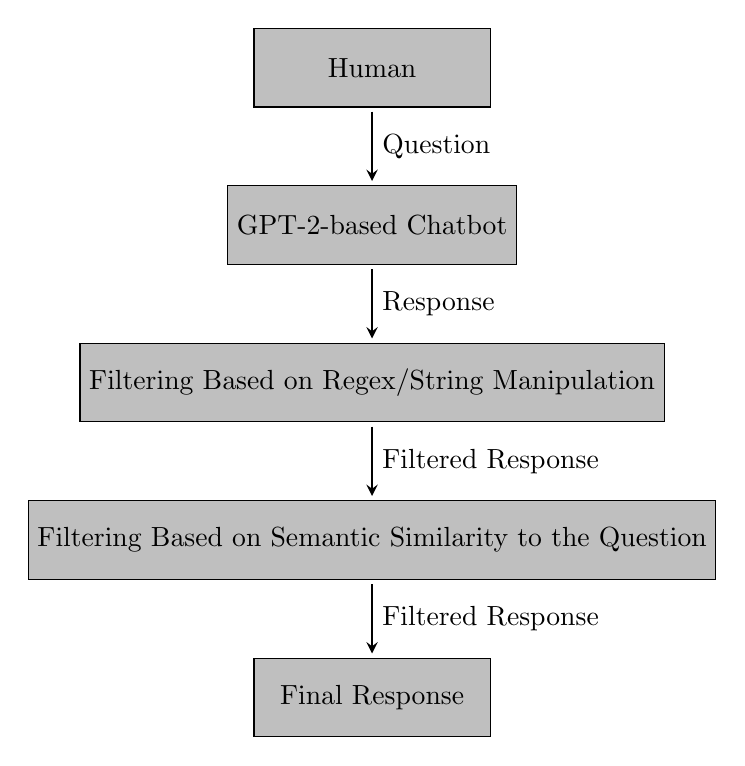
\begin{tikzpicture}[node distance=2cm]
    \node (human)        [item]                     {Human};
    \node (chatbot)      [item, below of=human]     {GPT-2-based Chatbot};
    \node (filtering)    [item, below of=chatbot]   {Filtering Based on Regex/String
      Manipulation};
    \node (filtering-ss) [item, below of=filtering] {Filtering Based on Semantic
      Similarity to the Question};
    \node (final)     [item, below of=filtering-ss] {Final Response};

    \draw [arrow] (human)        -- node[anchor=west] {Question}          (chatbot);
    \draw [arrow] (chatbot)      -- node[anchor=west] {Response}          (filtering);
    \draw [arrow] (filtering)    -- node[anchor=west] {Filtered Response} (filtering-ss);
    \draw [arrow] (filtering-ss) -- node[anchor=west] {Filtered Response} (final);
  \end{tikzpicture}
  \caption{Response Generation.}
\end{figure}

\subsection{Transfer Learning}

We utilized GPT-2 774M model and ran transfer learning for 2500 iterations with
the batch size of 8. We used Adam~\cite{adam} as the optimizer and set the
learning rate of 0.0001. The link for downloading the model is available on our
GitHub page.

\bigskip

\noindent GPT-2 has a Transformer~\cite{vaswani} based architecture which, in
many ways, is similar to Open AI GPT model\cite{radford2019language}\cite{gpt}.
There are 4 different versions of GPT-2. It features models with 124 million,
355 million, 774 million, and 1.5 billion parameters. We have utilized the
version with 774 million parameters. The original GPT-2 was written in
tensorflow~\cite{tensorflow2015-whitepaper} and this is the version we have
used. That said, for retraining purposes, we have utilized the TPU-trainable
version of the GPT-2~\cite{gpt-2-tpu}.

\bigskip

\noindent Adam an algorithm for first-order gradient-based optimization of
stochastic objective functions, based on adaptive estimates of lower-order
moments~\cite{adam}. It is highly memory-efficient and has shown good results
in retraining our chatbot. We have also tried SGD~\cite{SGD}, yet Adam has
shown a better performance and therefore, we have released the Adam-based
GPT-2 retrained model.

\bigskip

\noindent For building a web interface for our chatbot, we have used Python's
package flask~\cite{flask} and integrated it with tensorflow. This resulted
in a simple and user-friendly user interface.

%%%%%%%%%%%%%%%%%%%%%%%%%%%%%%%%%%%%%%%%%%%%%%%%%%%%%%%%%%%%%%%%%%%%%%%%%%%%%%%
% Semantic Similarity
%%%%%%%%%%%%%%%%%%%%%%%%%%%%%%%%%%%%%%%%%%%%%%%%%%%%%%%%%%%%%%%%%%%%%%%%%%%%%%%

\subsection{Semantic Similarity}

Semantic similarity is a metric that quantifies the degree to which two texts
or text documents are similar to each other. The two approaches we have used
include cosine similarity and inner product. We used these approaches as an
additional layer to the language model.

\bigskip

\noindent Cosine similarity is one of the most commonly used approaches in
calculating semantic similarity of texts. Therefore, it is naturally employed
in natural language processing tasks. Many NLP applications need to
compute the semantic similarity between two short texts. Its flexibility allows
one to apply it under virtually any settings, as long as documents can be
represented as vectors.  Besides, finding cosine similarity is usually not a
time-consuming task and can be done really quickly. Therefore, it is also commonly
used for benchmarking purposes~\cite{cosine-benchmark}.

\bigskip

\noindent The GPT-2 responses are usually very lengthy and for the most part,
the answer is not relevant to the question. To solve this problem, we chunked
the answer into separate sentences and found the ones that are most
\textit{semantically similar} to the question asked. For this task, we have
tested and applied 4 different approaches:

\begin{itemize}
  \item BioBERT large v1.1 (+PubMed 1M) model based on BERT-large Cased (custom 30k vocabulary)
  \item Universal Sentence Encoder (USE), version 3, large
  \item Bert-Large, uncased (24 layers and 340M parameters)
  \item Scikit learn's Tfidfvectorizer
\end{itemize}

\noindent Once the embeddings were generated, we have applied cosine similarity and in
some cases, inner product and took 5 most similar sentences. Some additional
regex and text filters were added for fixing punctuation and other grammar-related
errors.

%%%%%%%%%%%%%%%%%%%%%%%%%%%%%%%%%%%%%%%%%%%%%%%%%%%%%%%%%%%%%%%%%%%%%%%%%%%%%%%
% Questions and Evaluation
%%%%%%%%%%%%%%%%%%%%%%%%%%%%%%%%%%%%%%%%%%%%%%%%%%%%%%%%%%%%%%%%%%%%%%%%%%%%%%%

\section{Questions and Evaluation}

In order to evaluate the performance of the approaches as well as the overall
performance of the chatbot, it was important to have the questions that both
are frequently asked and linked to COVID-19. For this purpose, we decided to
use 12 questions from the Kaggle's COVID-19 Open Research Dataset Challenge
(CORD-19)~\cite{kaggle}. Most of the questions included a term ``COVID-19,''
but some did not, in which case we appended the term to the end of the
question. Figure 2 presents all 12 questions.

\newpage % Needed to avoid unwanted spaces

\begin{figure}[H]
  \small
  \begin{tabular}{p{0.1\linewidth}p{0.9\linewidth}}
    \toprule
    Number & Question\\
    \midrule
    \#1 & Are there geographic variations in the mortality rate of COVID-19?\\
    \midrule
    \#2 & What is known about transmission, incubation, and environmental
      stability of COVID-19?\\
    \midrule
    \#3 & Is there any evidence to suggest geographic based virus mutations of
      COVID-19?\\
    \midrule
    \#4 & Are there geographic variations in the rate of COVID-19 spread?\\
    \midrule
    \#5 & What do we know about virus genetics, origin, and evolution of
      COVID-19?\\
    \midrule
    \#6 & What has been published about ethical and social science considerations
      of COVID-19?\\
    \midrule
    \#7 & What has been published about medical care of COVID-19?\\
    \midrule
    \#8 & What do we know about diagnostics and surveillance of COVID-19?\\
    \midrule
    \#9 & What do we know about COVID-19 risk factors?\\
    \midrule
    \#10 & What has been published about information sharing and inter-sectoral
      collaboration of COVID-19?\\
    \midrule
    \#11 & What do we know about vaccines and therapeutics of COVID-19\\
    \midrule
    \#12 & What do we know about non-pharmaceutical interventions of COVID-19?\\
    \bottomrule
  \end{tabular}
  \caption{12 Questions from Kaggle.}
\end{figure}

\noindent For each approach, we generated 5 different answers for the same
question, resulting in the total of 240 answers. Additionally, we made all of
the answers publicly available on GitHub~\cite{github-results}. We then asked
experienced medical personnel at Mayo Clinic to rate these answers. The rating
system was composed of 5 different categories:

\begin{figure}[H]
  \small
  \begin{tabular}{p{0.2\linewidth}p{0.7\linewidth}p{0.1\linewidth}}
    \toprule
    Category & Description & Point(s)\\
    \midrule
    Relevant & The answer partially or fully answers the question and/or
      makes clear attempts to do so and is related to the question & 5\\
    \midrule
    Well-formed & the answer makes a logical sense and is somewhat related
      to both the question and COVID-19, yet it does not (partially or
      fully) answer the question & 4\\
    \midrule
    Informative & The answer is not related to the question, but provides
        some information about COVID-19 and makes a logical sense & 3\\
    \midrule
    Acceptable & The answer makes some logical sense and is weakly related   to the question or COVID-19, but is mostly difficult to understand &
      2\\
    \midrule
    Poor & the answer is totally unrelated to the question or COVID-19
      and/or does not make a logical sense & 2\\
    \bottomrule
  \end{tabular}
  \caption{5 Rating Categories.}
\end{figure}

\noindent Having 5 categories allowed for a flexibility of opinions and a broad range of scores which ultimately gave us a better way to evaluate
our chatbot.

%%%%%%%%%%%%%%%%%%%%%%%%%%%%%%%%%%%%%%%%%%%%%%%%%%%%%%%%%%%%%%%%%%%%%%%%%%%%%%%
% Results
%%%%%%%%%%%%%%%%%%%%%%%%%%%%%%%%%%%%%%%%%%%%%%%%%%%%%%%%%%%%%%%%%%%%%%%%%%%%%%%

\section{Results}

\subsection{General Performance.}

\begin{figure}[H]
  \small
  \begin{tabular}{*{3}{c}}
    \toprule
    Annotator & Approach & Score\\
    \midrule
    \#1 & TfidfVectorizer + Cosine Similarity & 3.909\\
    \midrule
    \#2 & TfidfVectorizer + Cosine Similarity & 3.727\\
    \midrule
    Average & TfidfVectorizer + Cosine Similarity & 3.818\\
    \midrule
    \#1 & BERT + Cosine Similarity & 4.182\\
    \midrule
    \#2 & BERT + Cosine Similarity & 4.309\\
    \midrule
    Average & BERT + Cosine Similarity & 4.246\\
    \midrule
    \#1 & BioBERT + Cosine Similarity & 4.167\\
    \midrule
    \#2 & BioBERT + Cosine Similarity & 4.093\\
    \midrule
    Average & BioBERT + Cosine Similarity & 4.130\\
    \midrule
    \#1 & Universal Sentence Encoder (USE) + Inner Product & 3.696\\
    \midrule
    \#2 & Universal Sentence Encoder (USE) + Inner Product & 4.125\\
    \midrule
    Average & Universal Sentence Encoder (USE) + Inner Product & 3.911\\
    \bottomrule
  \end{tabular}
  \caption{Comparison of 4 Different Approaches Across the Annotators.}
\end{figure}

\noindent The first annotator has rated BERT as the best approach with the
average score of 3.909. BioBERT has shown roughly the same performance (4.167),
with BERT rated slightly above. tf-idf procedure performed well, yet could not
outperform neither BERT nor BioBERT. USE had the worst performance out of all
embedding generation techniques with the score of 3.696 out of 5.

\bigskip

\noindent The second annotator, similarly, has given the highest average score
to BERT (4.309). USE comes the second with the score of 4.125 followed by
BioBERT with approximately the same score (4.093). tf-idf vectorization has
yielded the worst results.

\bigskip

\noindent In general, the results show the consistency across the annotators.
BERT and BioBERT have shown the best performance, with BERT being the leader.
Their average scores were 4.246 and 4.130 respectively. tf-idf (3.818) and USE
(3.911), on the other hand, have shown roughly similar, yet inferior to BERT
and BioBERT, performance. All four approaches, on average, can be considered to
be in the ``well-formed'' category with BERT and BioBERT being close to the
``Relevant'' category.


%%%%%%%%%%%%%%%%%%%%%%%%%%%%%%%%%%%%%%%%%%%%%%%%%%%%%%%%%%%%%%%%%%%%%%%%%%%%%%%
% Web Application
%%%%%%%%%%%%%%%%%%%%%%%%%%%%%%%%%%%%%%%%%%%%%%%%%%%%%%%%%%%%%%%%%%%%%%%%%%%%%%%

\section{Web Application}

In order to make the chatbot more accessible to the general audience as well as
for automating the response generation and facilitating information exchange,
we have built a web application for the chatbot~\cite{web-app}. The application
is powered by Python's flask~\cite{flask} package and gives a simple and
user-friendly means for an interactive communication with the chatbot. In other
words, any person could use this application to learn more about COVID-19 and
get answers to their questions on this topic. The image below shows the web
interface for the interactive chatbot.

\begin{figure}[H]
  \centering
  \frame{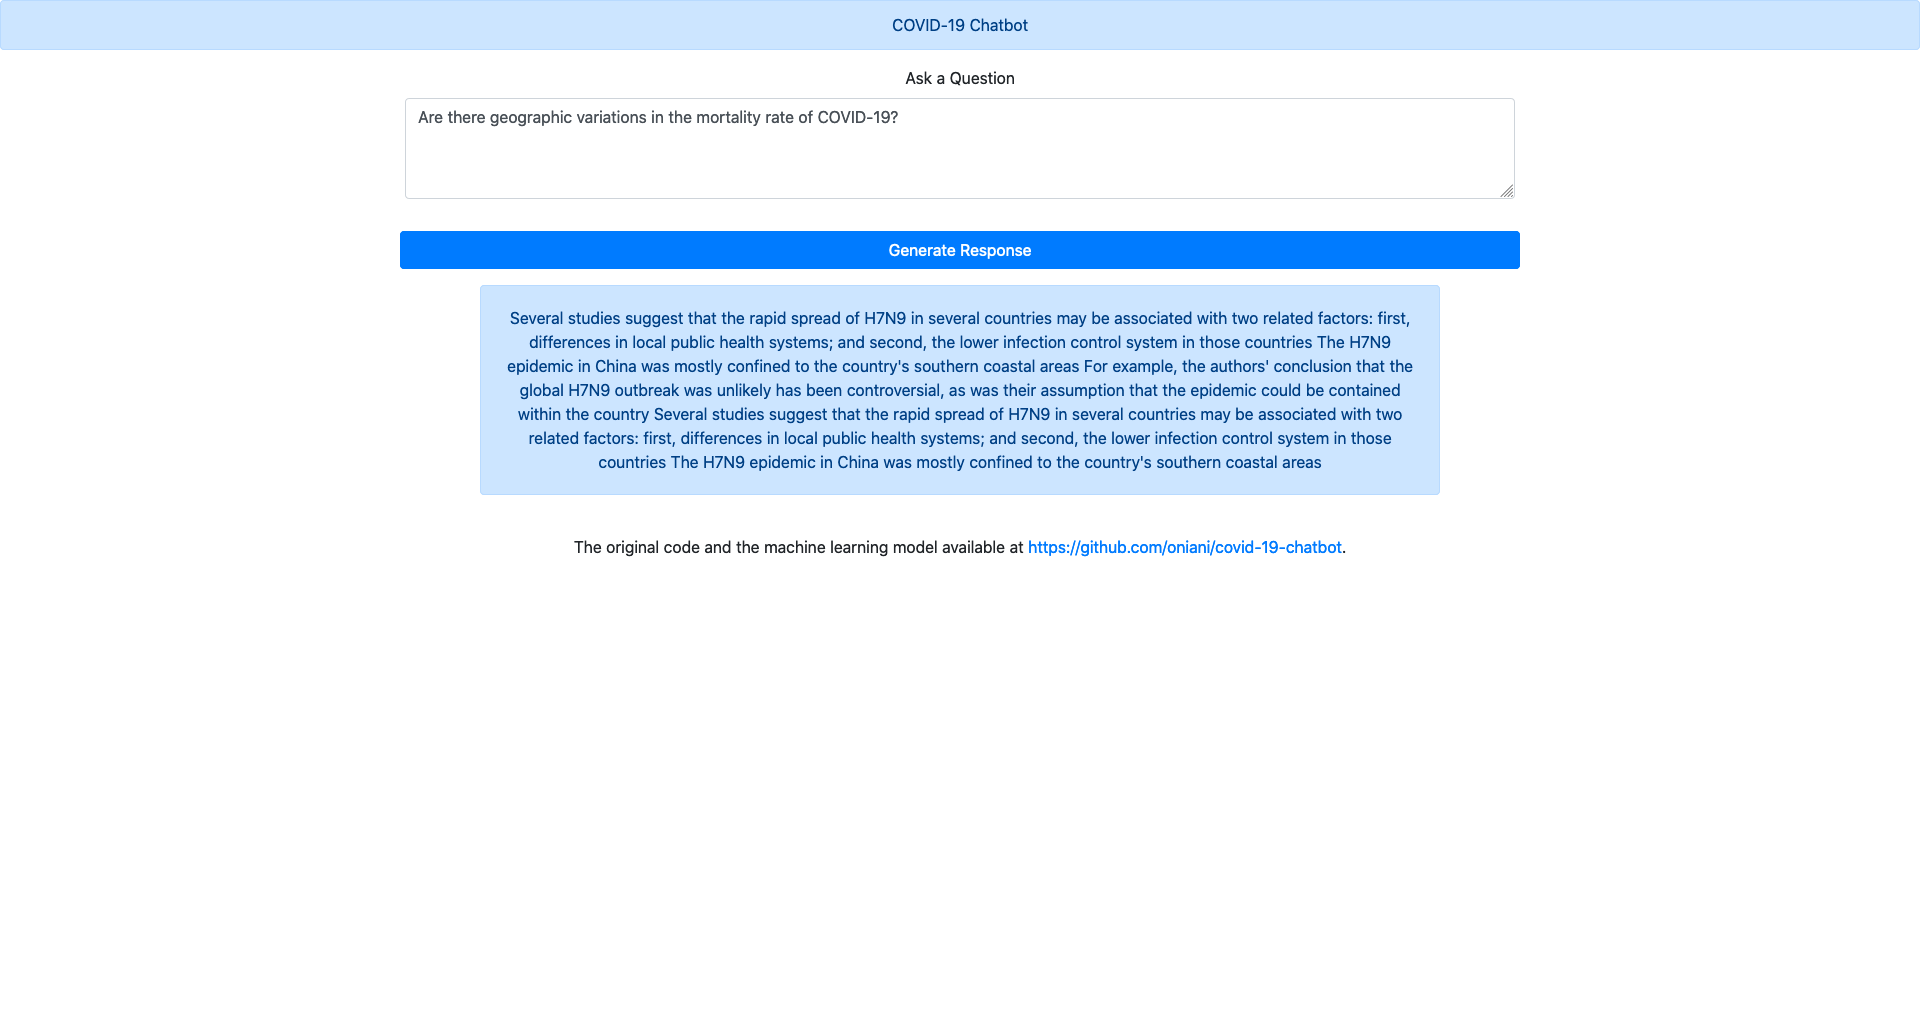
\includegraphics[width=\linewidth]{webapp.png}}
  \caption{An Image Depicting the Interactive Web Chatbot.}
\end{figure}


%%%%%%%%%%%%%%%%%%%%%%%%%%%%%%%%%%%%%%%%%%%%%%%%%%%%%%%%%%%%%%%%%%%%%%%%%%%%%%%
% Conclusion
%%%%%%%%%%%%%%%%%%%%%%%%%%%%%%%%%%%%%%%%%%%%%%%%%%%%%%%%%%%%%%%%%%%%%%%%%%%%%%%

\section{Conclusion}

We have explored the feasibility of utilizing GPT-2 for answering questions
related to COVID-19. GPT-2 was retrained on the CORD-19 corpus featuring
thousands of scholarly articles. Some of the example answers to the
COVID-19-related were made available online. Four different embedding
generation techniques (tf-idf, BERT, BioBERT, and Universal Sentence Encoder
(USE)) were compared.  The results were annotated by experienced medical staff
at Mayo Clinic. The annotation results were consistent and concluded that BERT
and BioBERT have the best average performance. USE came next with tf-idf
showing the worst average performance.

%%%%%%%%%%%%%%%%%%%%%%%%%%%%%%%%%%%%%%%%%%%%%%%%%%%%%%%%%%%%%%%%%%%%%%%%%%%%%%%
% References
%%%%%%%%%%%%%%%%%%%%%%%%%%%%%%%%%%%%%%%%%%%%%%%%%%%%%%%%%%%%%%%%%%%%%%%%%%%%%%%

\printbibliography%

\end{document}
